\begin{exe}
    \ex Andrew hits Mathis.
        \begin{xlist}
            \ex \begin{tikzpicture}[baseline=(top.base)]
                    \Tree [.\node(top){S }; [.NP^1 [.N^1 Andrew ] ] [.VP [.V hits ] [.NP^2 [.N^2 Mathis ] ] ] ]
                \end{tikzpicture}
            \ex \begin{tikzpicture}[baseline=(top.base)]
                    \Tree [.\node(top){S\,^{{\color{mygreen}\mathtt{FA\shortleftarrow}}}_{{\color{myred}t}} }; [.NP^1\,^{{\color{mygreen}\mathtt{NN}}}_{{\color{myred}e}} [.N^1\,^{{\color{mygreen}\mathtt{NN}}}_{{\color{myred}e}} Andrew\,^{{\color{mygreen}\mathtt{TN_1}}}_{{\color{myred}e}} ] ] [.VP\,^{{\color{mygreen}\mathtt{FA\shortrightarrow}}}_{{\color{myred}\langle e,\, t\rangle}} [.V\,^{{\color{mygreen}\mathtt{NN}}}_{{\color{myred}\langle e,\, \langle e,\, t\rangle\rangle}} hits\,^{{\color{mygreen}\mathtt{TN_1}}}_{{\color{myred}\langle e,\, \langle e,\, t\rangle\rangle}} ] [.NP^2\,^{{\color{mygreen}\mathtt{NN}}}_{{\color{myred}e}} [.N^2\,^{{\color{mygreen}\mathtt{NN}}}_{{\color{myred}e}} Mathis\,^{{\color{mygreen}\mathtt{TN_1}}}_{{\color{myred}e}} ] ] ] ]
                \end{tikzpicture}
        \end{xlist}
    \end{exe}

\begin{exe}
    \ex Not tanzt.
        \begin{xlist}
            \ex \begin{tikzpicture}[baseline=(top.base)]
                    \Tree [.\node(top){A }; [.B not [.C [.D [.E [.F [.G tanzt ] ] ] ] [.Peter ] ] ] ]
                \end{tikzpicture}
            \ex \begin{tikzpicture}[baseline=(top.base)]
                    \Tree [.\node(top){A\,^{{\color{mygreen}\mathtt{NN}}}_{{\color{myred}t}} }; [.B\,^{{\color{mygreen}\mathtt{FA\shortrightarrow}}}_{{\color{myred}t}} not\,^{{\color{mygreen}\mathtt{TN_1}}}_{{\color{myred}\langle t,\, t\rangle}} [.C\,^{{\color{mygreen}\mathtt{FA\shortrightarrow}}}_{{\color{myred}t}} [.D\,^{{\color{mygreen}\mathtt{NN}}}_{{\color{myred}\langle e,\, t\rangle}} [.E\,^{{\color{mygreen}\mathtt{NN}}}_{{\color{myred}\langle e,\, t\rangle}} [.F\,^{{\color{mygreen}\mathtt{NN}}}_{{\color{myred}\langle e,\, t\rangle}} [.G\,^{{\color{mygreen}\mathtt{NN}}}_{{\color{myred}\langle e,\, t\rangle}} tanzt\,^{{\color{mygreen}\mathtt{TN_1}}}_{{\color{myred}\langle e,\, t\rangle}} ] ] ] ] [.Peter\,^{{\color{mygreen}\mathtt{TN_1}}}_{{\color{myred}e}} ] ] ] ]
                \end{tikzpicture}
        \end{xlist}
    \end{exe}

\begin{exe}
    \ex Der große verschüchterte fliegende Wolf aus Twilight.
        \begin{xlist}
            \ex \begin{tikzpicture}[baseline=(top.base)]
                    \Tree [.\node(top){DP }; [.D der ] [.NP [.AP [.A große ] ] [.N$''''$ [.AP^2 [.A^2 verschüchterte ] ] [.N$'''$ [.AP^3 [.A^3 fliegende ] ] [.N$''$ [.N$'$ [.N Wolf ] ] [.PP [.P aus ] [.NP^2 [.N^2 Twilight ] ] ] ] ] ] ] ]
                \end{tikzpicture}
            \ex \begin{tikzpicture}[baseline=(top.base)]
                    \Tree [.\node(top){DP\,^{{\color{mygreen}\mathtt{FA\shortrightarrow}}}_{{\color{myred}e}} }; [.D\,^{{\color{mygreen}\mathtt{NN}}}_{{\color{myred}\langle \langle e,\, t\rangle,\, e\rangle}} der\,^{{\color{mygreen}\mathtt{TN_1}}}_{{\color{myred}\langle \langle e,\, t\rangle,\, e\rangle}} ] [.NP\,^{{\color{mygreen}\mathtt{PM}}}_{{\color{myred}\langle e,\, t\rangle}} [.AP\,^{{\color{mygreen}\mathtt{NN}}}_{{\color{myred}\langle e,\, t\rangle}} [.A\,^{{\color{mygreen}\mathtt{NN}}}_{{\color{myred}\langle e,\, t\rangle}} große\,^{{\color{mygreen}\mathtt{TN_1}}}_{{\color{myred}\langle e,\, t\rangle}} ] ] [.N$''''$\,^{{\color{mygreen}\mathtt{PM}}}_{{\color{myred}\langle e,\, t\rangle}} [.AP^2\,^{{\color{mygreen}\mathtt{NN}}}_{{\color{myred}\langle e,\, t\rangle}} [.A^2\,^{{\color{mygreen}\mathtt{NN}}}_{{\color{myred}\langle e,\, t\rangle}} verschüchterte\,^{{\color{mygreen}\mathtt{TN_1}}}_{{\color{myred}\langle e,\, t\rangle}} ] ] [.N$'''$\,^{{\color{mygreen}\mathtt{PM}}}_{{\color{myred}\langle e,\, t\rangle}} [.AP^3\,^{{\color{mygreen}\mathtt{NN}}}_{{\color{myred}\langle e,\, t\rangle}} [.A^3\,^{{\color{mygreen}\mathtt{NN}}}_{{\color{myred}\langle e,\, t\rangle}} fliegende\,^{{\color{mygreen}\mathtt{TN_1}}}_{{\color{myred}\langle e,\, t\rangle}} ] ] [.N$''$\,^{{\color{mygreen}\mathtt{PM}}}_{{\color{myred}\langle e,\, t\rangle}} [.N$'$\,^{{\color{mygreen}\mathtt{NN}}}_{{\color{myred}\langle e,\, t\rangle}} [.N\,^{{\color{mygreen}\mathtt{NN}}}_{{\color{myred}\langle e,\, t\rangle}} Wolf\,^{{\color{mygreen}\mathtt{TN_1}}}_{{\color{myred}\langle e,\, t\rangle}} ] ] [.PP\,^{{\color{mygreen}\mathtt{FA\shortrightarrow}}}_{{\color{myred}\langle e,\, t\rangle}} [.P\,^{{\color{mygreen}\mathtt{NN}}}_{{\color{myred}\langle e,\, \langle e,\, t\rangle\rangle}} aus\,^{{\color{mygreen}\mathtt{TN_1}}}_{{\color{myred}\langle e,\, \langle e,\, t\rangle\rangle}} ] [.NP^2\,^{{\color{mygreen}\mathtt{NN}}}_{{\color{myred}e}} [.N^2\,^{{\color{mygreen}\mathtt{NN}}}_{{\color{myred}e}} Twilight\,^{{\color{mygreen}\mathtt{TN_1}}}_{{\color{myred}e}} ] ] ] ] ] ] ] ]
                \end{tikzpicture}
        \end{xlist}
    \end{exe}

\begin{exe}
    \ex Andrew malt den Wolf und_{ind} die Blumen.
        \begin{xlist}
            \ex \begin{tikzpicture}[baseline=(top.base)]
                    \Tree [.\node(top){S }; [.NP [.N Andrew ] ] [.VP [.V malt ] [.CoordP [.DP^1 [.D^1 den ] [.NP^2 [.N^2 Wolf ] ] ] [.Coord$'$ [.Coord und_{ind} ] [.DP^2 [.D^2 die ] [.NP^3 [.N^3 Blumen ] ] ] ] ] ] ]
                \end{tikzpicture}
            \ex \begin{tikzpicture}[baseline=(top.base)]
                    \Tree [.\node(top){S\,^{{\color{mygreen}\mathtt{FA\shortleftarrow}}}_{{\color{myred}t}} }; [.NP\,^{{\color{mygreen}\mathtt{NN}}}_{{\color{myred}e}} [.N\,^{{\color{mygreen}\mathtt{NN}}}_{{\color{myred}e}} Andrew\,^{{\color{mygreen}\mathtt{TN_1}}}_{{\color{myred}e}} ] ] [.VP\,^{{\color{mygreen}\mathtt{FA\shortrightarrow}}}_{{\color{myred}\langle e,\, t\rangle}} [.V\,^{{\color{mygreen}\mathtt{NN}}}_{{\color{myred}\langle e,\, \langle e,\, t\rangle\rangle}} malt\,^{{\color{mygreen}\mathtt{TN_1}}}_{{\color{myred}\langle e,\, \langle e,\, t\rangle\rangle}} ] [.CoordP\,^{{\color{mygreen}\mathtt{FA\shortleftarrow}}}_{{\color{myred}e}} [.DP^1\,^{{\color{mygreen}\mathtt{FA\shortrightarrow}}}_{{\color{myred}e}} [.D^1\,^{{\color{mygreen}\mathtt{NN}}}_{{\color{myred}\langle \langle e,\, t\rangle,\, e\rangle}} den\,^{{\color{mygreen}\mathtt{TN_1}}}_{{\color{myred}\langle \langle e,\, t\rangle,\, e\rangle}} ] [.NP^2\,^{{\color{mygreen}\mathtt{NN}}}_{{\color{myred}\langle e,\, t\rangle}} [.N^2\,^{{\color{mygreen}\mathtt{NN}}}_{{\color{myred}\langle e,\, t\rangle}} Wolf\,^{{\color{mygreen}\mathtt{TN_1}}}_{{\color{myred}\langle e,\, t\rangle}} ] ] ] [.Coord$'$\,^{{\color{mygreen}\mathtt{FA\shortrightarrow}}}_{{\color{myred}\langle e,\, e\rangle}} [.Coord\,^{{\color{mygreen}\mathtt{NN}}}_{{\color{myred}\langle e,\, \langle e,\, e\rangle\rangle}} und_{ind}\,^{{\color{mygreen}\mathtt{TN_1}}}_{{\color{myred}\langle e,\, \langle e,\, e\rangle\rangle}} ] [.DP^2\,^{{\color{mygreen}\mathtt{FA\shortrightarrow}}}_{{\color{myred}e}} [.D^2\,^{{\color{mygreen}\mathtt{NN}}}_{{\color{myred}\langle \langle e,\, t\rangle,\, e\rangle}} die\,^{{\color{mygreen}\mathtt{TN_1}}}_{{\color{myred}\langle \langle e,\, t\rangle,\, e\rangle}} ] [.NP^3\,^{{\color{mygreen}\mathtt{NN}}}_{{\color{myred}\langle e,\, t\rangle}} [.N^3\,^{{\color{mygreen}\mathtt{NN}}}_{{\color{myred}\langle e,\, t\rangle}} Blumen\,^{{\color{mygreen}\mathtt{TN_1}}}_{{\color{myred}\langle e,\, t\rangle}} ] ] ] ] ] ] ]
                \end{tikzpicture}
        \end{xlist}
    \end{exe}

\begin{exe}
    \ex A person not Bill invite.
        \begin{xlist}
            \ex \begin{tikzpicture}[baseline=(top.base)]
                    \Tree [.\node(top){S }; [.DP [.D a ] [.NP [.N person ] ] ] [.XP [.1 ] [.S$'$ [.Neg not ] [.S$''$ [.NP^2 [.N^2 Bill ] ] [.VP [.V invite ] [.$t$ ] ] ] ] ] ]
                \end{tikzpicture}
            \ex \begin{tikzpicture}[baseline=(top.base)]
                    \Tree [.\node(top){S\,^{{\color{mygreen}\mathtt{FA\shortrightarrow}}}_{{\color{myred}t}} }; [.DP\,^{{\color{mygreen}\mathtt{FA\shortrightarrow}}}_{{\color{myred}\langle \langle e,\, t\rangle,\, t\rangle}} [.D\,^{{\color{mygreen}\mathtt{NN}}}_{{\color{myred}\langle \langle e,\, t\rangle,\, \langle \langle e,\, t\rangle,\, t\rangle\rangle}} a\,^{{\color{mygreen}\mathtt{TN_1}}}_{{\color{myred}\langle \langle e,\, t\rangle,\, \langle \langle e,\, t\rangle,\, t\rangle\rangle}} ] [.NP\,^{{\color{mygreen}\mathtt{NN}}}_{{\color{myred}\langle e,\, t\rangle}} [.N\,^{{\color{mygreen}\mathtt{NN}}}_{{\color{myred}\langle e,\, t\rangle}} person\,^{{\color{mygreen}\mathtt{TN_1}}}_{{\color{myred}\langle e,\, t\rangle}} ] ] ] [.XP\,^{{\color{mygreen}\mathtt{PA}}}_{{\color{myred}\langle e,\, t\rangle}} [.1\,^{{\color{mygreen}\mathtt{-}}}_{{\color{myred}-}} ] [.S$'$\,^{{\color{mygreen}\mathtt{FA\shortrightarrow}}}_{{\color{myred}t}} [.Neg\,^{{\color{mygreen}\mathtt{NN}}}_{{\color{myred}\langle t,\, t\rangle}} not\,^{{\color{mygreen}\mathtt{TN_1}}}_{{\color{myred}\langle t,\, t\rangle}} ] [.S$''$\,^{{\color{mygreen}\mathtt{FA\shortleftarrow}}}_{{\color{myred}t}} [.NP^2\,^{{\color{mygreen}\mathtt{NN}}}_{{\color{myred}e}} [.N^2\,^{{\color{mygreen}\mathtt{NN}}}_{{\color{myred}e}} Bill\,^{{\color{mygreen}\mathtt{TN_1}}}_{{\color{myred}e}} ] ] [.VP\,^{{\color{mygreen}\mathtt{FA\shortrightarrow}}}_{{\color{myred}\langle e,\, t\rangle}} [.V\,^{{\color{mygreen}\mathtt{NN}}}_{{\color{myred}\langle e,\, \langle e,\, t\rangle\rangle}} invite\,^{{\color{mygreen}\mathtt{TN_1}}}_{{\color{myred}\langle e,\, \langle e,\, t\rangle\rangle}} ] [.$t$\,^{{\color{mygreen}\mathtt{TN_2}}}_{{\color{myred}e}} ] ] ] ] ] ]
                \end{tikzpicture}
        \end{xlist}
    \end{exe}

\begin{exe}
    \ex Schuldiger Idiot.
        \begin{xlist}
            \ex 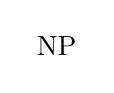
\begin{tikzpicture}[baseline=(top.base)]
                    \Tree [.\node(top){NP }; [.AP schuldiger ] [.N Idiot ] ]
                \end{tikzpicture}
            \ex \begin{tikzpicture}[baseline=(top.base)]
                    \Tree [.\node(top){NP\,^{{\color{mygreen}\mathtt{PM}}}_{{\color{myred}\langle e,\, t\rangle}} }; [.AP\,^{{\color{mygreen}\mathtt{NN}}}_{{\color{myred}\langle e,\, t\rangle}} schuldiger\,^{{\color{mygreen}\mathtt{TN_1}}}_{{\color{myred}\langle e,\, t\rangle}} ] [.N\,^{{\color{mygreen}\mathtt{NN}}}_{{\color{myred}\langle e,\, t\rangle}} Idiot\,^{{\color{mygreen}\mathtt{TN_1}}}_{{\color{myred}\langle e,\, t\rangle}} ] ]
                \end{tikzpicture}
        \end{xlist}
    \end{exe}

\begin{exe}
    \ex Some person is sad or she sleeps.
        \begin{xlist}
            \ex \begin{tikzpicture}[baseline=(top.base)]
                    \Tree [.\node(top){S }; [.S'' [.NP^1 [.Q some ] [.N^1 person ] ] [.VP [.V is ] [.AP [.A sad ] ] ] ] [.DisjP [.Disj or ] [.S' [.NP^2 [.N^2 she ] ] [.VP^2 [.V^2 sleeps ] ] ] ] ]
                \end{tikzpicture}
            \ex \begin{tikzpicture}[baseline=(top.base)]
                    \Tree [.\node(top){S\,^{{\color{mygreen}\mathtt{FA\shortleftarrow}}}_{{\color{myred}t}} }; [.S''\,^{{\color{mygreen}\mathtt{FA\shortrightarrow}}}_{{\color{myred}t}} [.NP^1\,^{{\color{mygreen}\mathtt{FA\shortrightarrow}}}_{{\color{myred}\langle \langle e,\, t\rangle,\, t\rangle}} [.Q\,^{{\color{mygreen}\mathtt{NN}}}_{{\color{myred}\langle \langle e,\, t\rangle,\, \langle \langle e,\, t\rangle,\, t\rangle\rangle}} some\,^{{\color{mygreen}\mathtt{TN_1}}}_{{\color{myred}\langle \langle e,\, t\rangle,\, \langle \langle e,\, t\rangle,\, t\rangle\rangle}} ] [.N^1\,^{{\color{mygreen}\mathtt{NN}}}_{{\color{myred}\langle e,\, t\rangle}} person\,^{{\color{mygreen}\mathtt{TN_1}}}_{{\color{myred}\langle e,\, t\rangle}} ] ] [.VP\,^{{\color{mygreen}\mathtt{NN}}}_{{\color{myred}\langle e,\, t\rangle}} [.V\,^{{\color{mygreen}\mathtt{NN}}}_{{\color{myred}-}} is\,^{{\color{mygreen}\mathtt{-}}}_{{\color{myred}-}} ] [.AP\,^{{\color{mygreen}\mathtt{NN}}}_{{\color{myred}\langle e,\, t\rangle}} [.A\,^{{\color{mygreen}\mathtt{NN}}}_{{\color{myred}\langle e,\, t\rangle}} sad\,^{{\color{mygreen}\mathtt{TN_1}}}_{{\color{myred}\langle e,\, t\rangle}} ] ] ] ] [.DisjP\,^{{\color{mygreen}\mathtt{FA\shortrightarrow}}}_{{\color{myred}\langle t,\, t\rangle}} [.Disj\,^{{\color{mygreen}\mathtt{NN}}}_{{\color{myred}\langle t,\, \langle t,\, t\rangle\rangle}} or\,^{{\color{mygreen}\mathtt{TN_1}}}_{{\color{myred}\langle t,\, \langle t,\, t\rangle\rangle}} ] [.S'\,^{{\color{mygreen}\mathtt{FA\shortleftarrow}}}_{{\color{myred}t}} [.NP^2\,^{{\color{mygreen}\mathtt{NN}}}_{{\color{myred}e}} [.N^2\,^{{\color{mygreen}\mathtt{NN}}}_{{\color{myred}e}} she\,^{{\color{mygreen}\mathtt{TN_2}}}_{{\color{myred}e}} ] ] [.VP^2\,^{{\color{mygreen}\mathtt{NN}}}_{{\color{myred}\langle e,\, t\rangle}} [.V^2\,^{{\color{mygreen}\mathtt{NN}}}_{{\color{myred}\langle e,\, t\rangle}} sleeps\,^{{\color{mygreen}\mathtt{TN_1}}}_{{\color{myred}\langle e,\, t\rangle}} ] ] ] ] ]
                \end{tikzpicture}
        \end{xlist}
    \end{exe}

\begin{exe}
    \ex Alle Blumen beobachtet Peter.
        \begin{xlist}
            \ex \begin{tikzpicture}[baseline=(top.base)]
                    \Tree [.\node(top){S' }; [.NP^1 [.Q alle ] [.N^1 Blumen ] ] [.XP [.1 ] [.S [.VP [.V beobachtet ] [.$t$ ] ] [.NP^2 [.N^2 Peter ] ] ] ] ]
                \end{tikzpicture}
            \ex \begin{tikzpicture}[baseline=(top.base)]
                    \Tree [.\node(top){S'\,^{{\color{mygreen}\mathtt{FA\shortrightarrow}}}_{{\color{myred}t}} }; [.NP^1\,^{{\color{mygreen}\mathtt{FA\shortrightarrow}}}_{{\color{myred}\langle \langle e,\, t\rangle,\, t\rangle}} [.Q\,^{{\color{mygreen}\mathtt{NN}}}_{{\color{myred}\langle \langle e,\, t\rangle,\, \langle \langle e,\, t\rangle,\, t\rangle\rangle}} alle\,^{{\color{mygreen}\mathtt{TN_1}}}_{{\color{myred}\langle \langle e,\, t\rangle,\, \langle \langle e,\, t\rangle,\, t\rangle\rangle}} ] [.N^1\,^{{\color{mygreen}\mathtt{NN}}}_{{\color{myred}\langle e,\, t\rangle}} Blumen\,^{{\color{mygreen}\mathtt{TN_1}}}_{{\color{myred}\langle e,\, t\rangle}} ] ] [.XP\,^{{\color{mygreen}\mathtt{PA}}}_{{\color{myred}\langle e,\, t\rangle}} [.1\,^{{\color{mygreen}\mathtt{-}}}_{{\color{myred}-}} ] [.S\,^{{\color{mygreen}\mathtt{FA\shortrightarrow}}}_{{\color{myred}t}} [.VP\,^{{\color{mygreen}\mathtt{FA\shortrightarrow}}}_{{\color{myred}\langle e,\, t\rangle}} [.V\,^{{\color{mygreen}\mathtt{NN}}}_{{\color{myred}\langle e,\, \langle e,\, t\rangle\rangle}} beobachtet\,^{{\color{mygreen}\mathtt{TN_1}}}_{{\color{myred}\langle e,\, \langle e,\, t\rangle\rangle}} ] [.$t$\,^{{\color{mygreen}\mathtt{TN_2}}}_{{\color{myred}e}} ] ] [.NP^2\,^{{\color{mygreen}\mathtt{NN}}}_{{\color{myred}e}} [.N^2\,^{{\color{mygreen}\mathtt{NN}}}_{{\color{myred}e}} Peter\,^{{\color{mygreen}\mathtt{TN_1}}}_{{\color{myred}e}} ] ] ] ] ]
                \end{tikzpicture}
        \end{xlist}
    \end{exe}

\begin{exe}
    \ex Peter ist ein fliegender Junge aus Nimmerland.
        \begin{xlist}
            \ex \begin{tikzpicture}[baseline=(top.base)]
                    \Tree [.\node(top){S }; [.NP^1 [.N^1 Peter ] ] [.VP [.V ist ] [.DP [.D ein ] [.NP^2 [.N$''$^2 [.AP [.A fliegender ] ] [.N$'$^2 [.N^2 Junge ] ] ] [.PP [.P aus ] [.NP^3 [.N^3 Nimmerland ] ] ] ] ] ] ]
                \end{tikzpicture}
            \ex \begin{tikzpicture}[baseline=(top.base)]
                    \Tree [.\node(top){S\,^{{\color{mygreen}\mathtt{FA\shortleftarrow}}}_{{\color{myred}t}} }; [.NP^1\,^{{\color{mygreen}\mathtt{NN}}}_{{\color{myred}e}} [.N^1\,^{{\color{mygreen}\mathtt{NN}}}_{{\color{myred}e}} Peter\,^{{\color{mygreen}\mathtt{TN_1}}}_{{\color{myred}e}} ] ] [.VP\,^{{\color{mygreen}\mathtt{NN}}}_{{\color{myred}\langle e,\, t\rangle}} [.V\,^{{\color{mygreen}\mathtt{NN}}}_{{\color{myred}-}} ist\,^{{\color{mygreen}\mathtt{-}}}_{{\color{myred}-}} ] [.DP\,^{{\color{mygreen}\mathtt{NN}}}_{{\color{myred}\langle e,\, t\rangle}} [.D\,^{{\color{mygreen}\mathtt{NN}}}_{{\color{myred}-}} ein\,^{{\color{mygreen}\mathtt{-}}}_{{\color{myred}-}} ] [.NP^2\,^{{\color{mygreen}\mathtt{PM}}}_{{\color{myred}\langle e,\, t\rangle}} [.N$''$^2\,^{{\color{mygreen}\mathtt{PM}}}_{{\color{myred}\langle e,\, t\rangle}} [.AP\,^{{\color{mygreen}\mathtt{NN}}}_{{\color{myred}\langle e,\, t\rangle}} [.A\,^{{\color{mygreen}\mathtt{NN}}}_{{\color{myred}\langle e,\, t\rangle}} fliegender\,^{{\color{mygreen}\mathtt{TN_1}}}_{{\color{myred}\langle e,\, t\rangle}} ] ] [.N$'$^2\,^{{\color{mygreen}\mathtt{NN}}}_{{\color{myred}\langle e,\, t\rangle}} [.N^2\,^{{\color{mygreen}\mathtt{NN}}}_{{\color{myred}\langle e,\, t\rangle}} Junge\,^{{\color{mygreen}\mathtt{TN_1}}}_{{\color{myred}\langle e,\, t\rangle}} ] ] ] [.PP\,^{{\color{mygreen}\mathtt{FA\shortrightarrow}}}_{{\color{myred}\langle e,\, t\rangle}} [.P\,^{{\color{mygreen}\mathtt{NN}}}_{{\color{myred}\langle e,\, \langle e,\, t\rangle\rangle}} aus\,^{{\color{mygreen}\mathtt{TN_1}}}_{{\color{myred}\langle e,\, \langle e,\, t\rangle\rangle}} ] [.NP^3\,^{{\color{mygreen}\mathtt{NN}}}_{{\color{myred}e}} [.N^3\,^{{\color{mygreen}\mathtt{NN}}}_{{\color{myred}e}} Nimmerland\,^{{\color{mygreen}\mathtt{TN_1}}}_{{\color{myred}e}} ] ] ] ] ] ] ]
                \end{tikzpicture}
        \end{xlist}
    \end{exe}

\begin{exe}
    \ex Er ist stolz auf Maria.
        \begin{xlist}
            \ex \begin{tikzpicture}[baseline=(top.base)]
                    \Tree [.\node(top){S }; [.NP [.N er ] ] [.VP [.V ist ] [.AP [.A stolz ] [.PP [.P auf ] [.NP^2 [.N^2 Maria ] ] ] ] ] ]
                \end{tikzpicture}
            \ex \begin{tikzpicture}[baseline=(top.base)]
                    \Tree [.\node(top){S\,^{{\color{mygreen}\mathtt{FA\shortleftarrow}}}_{{\color{myred}t}} }; [.NP\,^{{\color{mygreen}\mathtt{NN}}}_{{\color{myred}e}} [.N\,^{{\color{mygreen}\mathtt{NN}}}_{{\color{myred}e}} er\,^{{\color{mygreen}\mathtt{TN_2}}}_{{\color{myred}e}} ] ] [.VP\,^{{\color{mygreen}\mathtt{NN}}}_{{\color{myred}\langle e,\, t\rangle}} [.V\,^{{\color{mygreen}\mathtt{NN}}}_{{\color{myred}-}} ist\,^{{\color{mygreen}\mathtt{-}}}_{{\color{myred}-}} ] [.AP\,^{{\color{mygreen}\mathtt{FA\shortrightarrow}}}_{{\color{myred}\langle e,\, t\rangle}} [.A\,^{{\color{mygreen}\mathtt{NN}}}_{{\color{myred}\langle e,\, \langle e,\, t\rangle\rangle}} stolz\,^{{\color{mygreen}\mathtt{TN_1}}}_{{\color{myred}\langle e,\, \langle e,\, t\rangle\rangle}} ] [.PP\,^{{\color{mygreen}\mathtt{NN}}}_{{\color{myred}e}} [.P\,^{{\color{mygreen}\mathtt{NN}}}_{{\color{myred}-}} auf\,^{{\color{mygreen}\mathtt{-}}}_{{\color{myred}-}} ] [.NP^2\,^{{\color{mygreen}\mathtt{NN}}}_{{\color{myred}e}} [.N^2\,^{{\color{mygreen}\mathtt{NN}}}_{{\color{myred}e}} Maria\,^{{\color{mygreen}\mathtt{TN_1}}}_{{\color{myred}e}} ] ] ] ] ] ]
                \end{tikzpicture}
        \end{xlist}
    \end{exe}

\begin{exe}
    \ex Einige schnarchende Jungen zwicken die kleinen Männer.
        \begin{xlist}
            \ex \begin{tikzpicture}[baseline=(top.base)]
                    \Tree [.\node(top){S }; [.NP [.Q einige ] [.N' [.AP^1 [.A^1 schnarchende ] ] [.N'' [.N Jungen ] ] ] ] [.VP [.V zwicken ] [.NP^2 [.D die ] [.N'^2 [.AP^2 [.A^2 kleinen ] ] [.N^2 Männer ] ] ] ] ]
                \end{tikzpicture}
            \ex \begin{tikzpicture}[baseline=(top.base)]
                    \Tree [.\node(top){S\,^{{\color{mygreen}\mathtt{FA\shortrightarrow}}}_{{\color{myred}t}} }; [.NP\,^{{\color{mygreen}\mathtt{FA\shortrightarrow}}}_{{\color{myred}\langle \langle e,\, t\rangle,\, t\rangle}} [.Q\,^{{\color{mygreen}\mathtt{NN}}}_{{\color{myred}\langle \langle e,\, t\rangle,\, \langle \langle e,\, t\rangle,\, t\rangle\rangle}} einige\,^{{\color{mygreen}\mathtt{TN_1}}}_{{\color{myred}\langle \langle e,\, t\rangle,\, \langle \langle e,\, t\rangle,\, t\rangle\rangle}} ] [.N'\,^{{\color{mygreen}\mathtt{PM}}}_{{\color{myred}\langle e,\, t\rangle}} [.AP^1\,^{{\color{mygreen}\mathtt{NN}}}_{{\color{myred}\langle e,\, t\rangle}} [.A^1\,^{{\color{mygreen}\mathtt{NN}}}_{{\color{myred}\langle e,\, t\rangle}} schnarchende\,^{{\color{mygreen}\mathtt{TN_1}}}_{{\color{myred}\langle e,\, t\rangle}} ] ] [.N''\,^{{\color{mygreen}\mathtt{NN}}}_{{\color{myred}\langle e,\, t\rangle}} [.N\,^{{\color{mygreen}\mathtt{NN}}}_{{\color{myred}\langle e,\, t\rangle}} Jungen\,^{{\color{mygreen}\mathtt{TN_1}}}_{{\color{myred}\langle e,\, t\rangle}} ] ] ] ] [.VP\,^{{\color{mygreen}\mathtt{FA\shortrightarrow}}}_{{\color{myred}\langle e,\, t\rangle}} [.V\,^{{\color{mygreen}\mathtt{NN}}}_{{\color{myred}\langle e,\, \langle e,\, t\rangle\rangle}} zwicken\,^{{\color{mygreen}\mathtt{TN_1}}}_{{\color{myred}\langle e,\, \langle e,\, t\rangle\rangle}} ] [.NP^2\,^{{\color{mygreen}\mathtt{FA\shortrightarrow}}}_{{\color{myred}e}} [.D\,^{{\color{mygreen}\mathtt{NN}}}_{{\color{myred}\langle \langle e,\, t\rangle,\, e\rangle}} die\,^{{\color{mygreen}\mathtt{TN_1}}}_{{\color{myred}\langle \langle e,\, t\rangle,\, e\rangle}} ] [.N'^2\,^{{\color{mygreen}\mathtt{PM}}}_{{\color{myred}\langle e,\, t\rangle}} [.AP^2\,^{{\color{mygreen}\mathtt{NN}}}_{{\color{myred}\langle e,\, t\rangle}} [.A^2\,^{{\color{mygreen}\mathtt{NN}}}_{{\color{myred}\langle e,\, t\rangle}} kleinen\,^{{\color{mygreen}\mathtt{TN_1}}}_{{\color{myred}\langle e,\, t\rangle}} ] ] [.N^2\,^{{\color{mygreen}\mathtt{NN}}}_{{\color{myred}\langle e,\, t\rangle}} Männer\,^{{\color{mygreen}\mathtt{TN_1}}}_{{\color{myred}\langle e,\, t\rangle}} ] ] ] ] ]
                \end{tikzpicture}
        \end{xlist}
    \end{exe}

\begin{exe}
    \ex Der Junge der_{RP} wo die Fee aus Nimmerland belästigt fliegt.
        \begin{xlist}
            \ex \begin{tikzpicture}[baseline=(top.base)]
                    \Tree [.\node(top){S }; [.DP^1 [.D^1 der ] [.NP [.N$''$ [.N$'$ [.N Junge ] ] [.CP [.DP^2 der_{RP} ] [.C$'$ [.C wo ] [.S$'$ [.$t$ ] [.VP [.DP^3 [.D^3 die ] [.NP^2 [.N$''$^2 [.N$'$^2 [.N^2 Fee ] ] [.PP [.P aus ] [.DP^4 Nimmerland ] ] ] ] ]  [.V belästigt ] ] ] ] ] ] ] ]  [.VP^2 [.V^2 fliegt ] ] ]
                \end{tikzpicture}
            \ex \begin{tikzpicture}[baseline=(top.base)]
                    \Tree [.\node(top){S\,^{{\color{mygreen}\mathtt{FA\shortleftarrow}}}_{{\color{myred}t}} }; [.DP^1\,^{{\color{mygreen}\mathtt{FA\shortrightarrow}}}_{{\color{myred}e}} [.D^1\,^{{\color{mygreen}\mathtt{NN}}}_{{\color{myred}\langle \langle e,\, t\rangle,\, e\rangle}} der\,^{{\color{mygreen}\mathtt{TN_1}}}_{{\color{myred}\langle \langle e,\, t\rangle,\, e\rangle}} ] [.NP\,^{{\color{mygreen}\mathtt{NN}}}_{{\color{myred}\langle e,\, t\rangle}} [.N$''$\,^{{\color{mygreen}\mathtt{PM}}}_{{\color{myred}\langle e,\, t\rangle}} [.N$'$\,^{{\color{mygreen}\mathtt{NN}}}_{{\color{myred}\langle e,\, t\rangle}} [.N\,^{{\color{mygreen}\mathtt{NN}}}_{{\color{myred}\langle e,\, t\rangle}} Junge\,^{{\color{mygreen}\mathtt{TN_1}}}_{{\color{myred}\langle e,\, t\rangle}} ] ] [.CP\,^{{\color{mygreen}\mathtt{PA}}}_{{\color{myred}\langle e,\, t\rangle}} [.DP^2\,^{{\color{mygreen}\mathtt{NN}}}_{{\color{myred}-}} der_{RP}\,^{{\color{mygreen}\mathtt{-}}}_{{\color{myred}-}} ] [.C$'$\,^{{\color{mygreen}\mathtt{NN}}}_{{\color{myred}t}} [.C\,^{{\color{mygreen}\mathtt{NN}}}_{{\color{myred}-}} wo\,^{{\color{mygreen}\mathtt{-}}}_{{\color{myred}-}} ] [.S$'$\,^{{\color{mygreen}\mathtt{FA\shortleftarrow}}}_{{\color{myred}t}} [.$t$\,^{{\color{mygreen}\mathtt{TN_2}}}_{{\color{myred}e}} ] [.VP\,^{{\color{mygreen}\mathtt{FA\shortleftarrow}}}_{{\color{myred}\langle e,\, t\rangle}} [.DP^3\,^{{\color{mygreen}\mathtt{FA\shortrightarrow}}}_{{\color{myred}e}} [.D^3\,^{{\color{mygreen}\mathtt{NN}}}_{{\color{myred}\langle \langle e,\, t\rangle,\, e\rangle}} die\,^{{\color{mygreen}\mathtt{TN_1}}}_{{\color{myred}\langle \langle e,\, t\rangle,\, e\rangle}} ] [.NP^2\,^{{\color{mygreen}\mathtt{NN}}}_{{\color{myred}\langle e,\, t\rangle}} [.N$''$^2\,^{{\color{mygreen}\mathtt{PM}}}_{{\color{myred}\langle e,\, t\rangle}} [.N$'$^2\,^{{\color{mygreen}\mathtt{NN}}}_{{\color{myred}\langle e,\, t\rangle}} [.N^2\,^{{\color{mygreen}\mathtt{NN}}}_{{\color{myred}\langle e,\, t\rangle}} Fee\,^{{\color{mygreen}\mathtt{TN_1}}}_{{\color{myred}\langle e,\, t\rangle}} ] ] [.PP\,^{{\color{mygreen}\mathtt{FA\shortrightarrow}}}_{{\color{myred}\langle e,\, t\rangle}} [.P\,^{{\color{mygreen}\mathtt{NN}}}_{{\color{myred}\langle e,\, \langle e,\, t\rangle\rangle}} aus\,^{{\color{mygreen}\mathtt{TN_1}}}_{{\color{myred}\langle e,\, \langle e,\, t\rangle\rangle}} ] [.DP^4\,^{{\color{mygreen}\mathtt{NN}}}_{{\color{myred}e}} Nimmerland\,^{{\color{mygreen}\mathtt{TN_1}}}_{{\color{myred}e}} ] ] ] ] ]  [.V\,^{{\color{mygreen}\mathtt{NN}}}_{{\color{myred}\langle e,\, \langle e,\, t\rangle\rangle}} belästigt\,^{{\color{mygreen}\mathtt{TN_1}}}_{{\color{myred}\langle e,\, \langle e,\, t\rangle\rangle}} ] ] ] ] ] ] ] ]  [.VP^2\,^{{\color{mygreen}\mathtt{NN}}}_{{\color{myred}\langle e,\, t\rangle}} [.V^2\,^{{\color{mygreen}\mathtt{NN}}}_{{\color{myred}\langle e,\, t\rangle}} fliegt\,^{{\color{mygreen}\mathtt{TN_1}}}_{{\color{myred}\langle e,\, t\rangle}} ] ] ]
                \end{tikzpicture}
        \end{xlist}
    \end{exe}

\begin{exe}
    \ex Dem Schüler das Buch Bill gibt.
        \begin{xlist}
            \ex \begin{tikzpicture}[baseline=(top.base)]
                    \Tree [.\node(top){WP }; [.DP^2 [.D^2 dem ] [.NP^2 [.N^2 Schüler ] ] ] [.ZP [.2 ] [.XP [.DP^1 [.D^1 das ] [.NP^1 [.N^1 Buch ] ] ] [.YP [.1 ] [.S [.NP^3 [.N^3 Bill ] ] [.VP [.V$'$ [.V gibt ] [.$t$ ] ] [.$t$ ] ] ] ] ] ] ]
                \end{tikzpicture}
            \ex \begin{tikzpicture}[baseline=(top.base)]
                    \Tree [.\node(top){WP\,^{{\color{mygreen}\mathtt{FA\shortleftarrow}}}_{{\color{myred}t}} }; [.DP^2\,^{{\color{mygreen}\mathtt{FA\shortrightarrow}}}_{{\color{myred}e}} [.D^2\,^{{\color{mygreen}\mathtt{NN}}}_{{\color{myred}\langle \langle e,\, t\rangle,\, e\rangle}} dem\,^{{\color{mygreen}\mathtt{TN_1}}}_{{\color{myred}\langle \langle e,\, t\rangle,\, e\rangle}} ] [.NP^2\,^{{\color{mygreen}\mathtt{NN}}}_{{\color{myred}\langle e,\, t\rangle}} [.N^2\,^{{\color{mygreen}\mathtt{NN}}}_{{\color{myred}\langle e,\, t\rangle}} Schüler\,^{{\color{mygreen}\mathtt{TN_1}}}_{{\color{myred}\langle e,\, t\rangle}} ] ] ] [.ZP\,^{{\color{mygreen}\mathtt{PA}}}_{{\color{myred}\langle e,\, t\rangle}} [.2\,^{{\color{mygreen}\mathtt{-}}}_{{\color{myred}-}} ] [.XP\,^{{\color{mygreen}\mathtt{FA\shortleftarrow}}}_{{\color{myred}t}} [.DP^1\,^{{\color{mygreen}\mathtt{FA\shortrightarrow}}}_{{\color{myred}e}} [.D^1\,^{{\color{mygreen}\mathtt{NN}}}_{{\color{myred}\langle \langle e,\, t\rangle,\, e\rangle}} das\,^{{\color{mygreen}\mathtt{TN_1}}}_{{\color{myred}\langle \langle e,\, t\rangle,\, e\rangle}} ] [.NP^1\,^{{\color{mygreen}\mathtt{NN}}}_{{\color{myred}\langle e,\, t\rangle}} [.N^1\,^{{\color{mygreen}\mathtt{NN}}}_{{\color{myred}\langle e,\, t\rangle}} Buch\,^{{\color{mygreen}\mathtt{TN_1}}}_{{\color{myred}\langle e,\, t\rangle}} ] ] ] [.YP\,^{{\color{mygreen}\mathtt{PA}}}_{{\color{myred}\langle e,\, t\rangle}} [.1\,^{{\color{mygreen}\mathtt{-}}}_{{\color{myred}-}} ] [.S\,^{{\color{mygreen}\mathtt{FA\shortleftarrow}}}_{{\color{myred}t}} [.NP^3\,^{{\color{mygreen}\mathtt{NN}}}_{{\color{myred}e}} [.N^3\,^{{\color{mygreen}\mathtt{NN}}}_{{\color{myred}e}} Bill\,^{{\color{mygreen}\mathtt{TN_1}}}_{{\color{myred}e}} ] ] [.VP\,^{{\color{mygreen}\mathtt{FA\shortrightarrow}}}_{{\color{myred}\langle e,\, t\rangle}} [.V$'$\,^{{\color{mygreen}\mathtt{FA\shortrightarrow}}}_{{\color{myred}\langle e,\, \langle e,\, t\rangle\rangle}} [.V\,^{{\color{mygreen}\mathtt{NN}}}_{{\color{myred}\langle e,\, \langle e,\, \langle e,\, t\rangle\rangle\rangle}} gibt\,^{{\color{mygreen}\mathtt{TN_1}}}_{{\color{myred}\langle e,\, \langle e,\, \langle e,\, t\rangle\rangle\rangle}} ] [.$t$\,^{{\color{mygreen}\mathtt{TN_2}}}_{{\color{myred}e}} ] ] [.$t$\,^{{\color{mygreen}\mathtt{TN_2}}}_{{\color{myred}e}} ] ] ] ] ] ] ]
                \end{tikzpicture}
        \end{xlist}
    \end{exe}

\begin{exe}
    \ex Alle Hunde einige Türen schließen.
        \begin{xlist}
            \ex \begin{tikzpicture}[baseline=(top.base)]
                    \Tree [.\node(top){S$'$ }; [.DP^2 [.D^2 alle ] [.NP^2 [.N^2 Hunde ] ] ] [.XP [.2 ] [.YP [.DP^1 [.D^1 einige ] [.NP^1 [.N^1 Türen ] ] ] [.ZP [.1 ] [.S [.$t$ ] [.VP [.V schließen ] [.$t$ ] ] ] ] ] ] ]
                \end{tikzpicture}
            \ex \begin{tikzpicture}[baseline=(top.base)]
                    \Tree [.\node(top){S$'$\,^{{\color{mygreen}\mathtt{FA\shortrightarrow}}}_{{\color{myred}t}} }; [.DP^2\,^{{\color{mygreen}\mathtt{FA\shortrightarrow}}}_{{\color{myred}\langle \langle e,\, t\rangle,\, t\rangle}} [.D^2\,^{{\color{mygreen}\mathtt{NN}}}_{{\color{myred}\langle \langle e,\, t\rangle,\, \langle \langle e,\, t\rangle,\, t\rangle\rangle}} alle\,^{{\color{mygreen}\mathtt{TN_1}}}_{{\color{myred}\langle \langle e,\, t\rangle,\, \langle \langle e,\, t\rangle,\, t\rangle\rangle}} ] [.NP^2\,^{{\color{mygreen}\mathtt{NN}}}_{{\color{myred}\langle e,\, t\rangle}} [.N^2\,^{{\color{mygreen}\mathtt{NN}}}_{{\color{myred}\langle e,\, t\rangle}} Hunde\,^{{\color{mygreen}\mathtt{TN_1}}}_{{\color{myred}\langle e,\, t\rangle}} ] ] ] [.XP\,^{{\color{mygreen}\mathtt{PA}}}_{{\color{myred}\langle e,\, t\rangle}} [.2\,^{{\color{mygreen}\mathtt{-}}}_{{\color{myred}-}} ] [.YP\,^{{\color{mygreen}\mathtt{FA\shortrightarrow}}}_{{\color{myred}t}} [.DP^1\,^{{\color{mygreen}\mathtt{FA\shortrightarrow}}}_{{\color{myred}\langle \langle e,\, t\rangle,\, t\rangle}} [.D^1\,^{{\color{mygreen}\mathtt{NN}}}_{{\color{myred}\langle \langle e,\, t\rangle,\, \langle \langle e,\, t\rangle,\, t\rangle\rangle}} einige\,^{{\color{mygreen}\mathtt{TN_1}}}_{{\color{myred}\langle \langle e,\, t\rangle,\, \langle \langle e,\, t\rangle,\, t\rangle\rangle}} ] [.NP^1\,^{{\color{mygreen}\mathtt{NN}}}_{{\color{myred}\langle e,\, t\rangle}} [.N^1\,^{{\color{mygreen}\mathtt{NN}}}_{{\color{myred}\langle e,\, t\rangle}} Türen\,^{{\color{mygreen}\mathtt{TN_1}}}_{{\color{myred}\langle e,\, t\rangle}} ] ] ] [.ZP\,^{{\color{mygreen}\mathtt{PA}}}_{{\color{myred}\langle e,\, t\rangle}} [.1\,^{{\color{mygreen}\mathtt{-}}}_{{\color{myred}-}} ] [.S\,^{{\color{mygreen}\mathtt{FA\shortleftarrow}}}_{{\color{myred}t}} [.$t$\,^{{\color{mygreen}\mathtt{TN_2}}}_{{\color{myred}e}} ] [.VP\,^{{\color{mygreen}\mathtt{FA\shortrightarrow}}}_{{\color{myred}\langle e,\, t\rangle}} [.V\,^{{\color{mygreen}\mathtt{NN}}}_{{\color{myred}\langle e,\, \langle e,\, t\rangle\rangle}} schließen\,^{{\color{mygreen}\mathtt{TN_1}}}_{{\color{myred}\langle e,\, \langle e,\, t\rangle\rangle}} ] [.$t$\,^{{\color{mygreen}\mathtt{TN_2}}}_{{\color{myred}e}} ] ] ] ] ] ] ]
                \end{tikzpicture}
        \end{xlist}
    \end{exe}

